\documentclass[12pt]{article}% uses letterpaper by default

%---------- Uncomment one of them ------------------------------
\usepackage[includeheadfoot, top=0.5in, bottom=0.5in, hmargin=1in]{geometry}

% \usepackage[a5paper, landscape, twocolumn, twoside,
%    left=2cm, hmarginratio=2:1, includemp, marginparwidth=43pt,
%    bottom=1cm, foot=.7cm, includefoot, textheight=11cm, heightrounded,
%    columnsep=1cm, dvips,  verbose]{geometry}
%---------------------------------------------------------------
\usepackage{fancyhdr}
\usepackage{setspace}
\renewcommand{\footrulewidth}{0.4pt}% default is 0pt
\usepackage[makeroom]{cancel}
\pagestyle{fancy}
\usepackage{graphicx}
\singlespacing
\usepackage{amsmath}

% \newcommand{}{\vspace{6em}}
\newcommand{\degrees}{\ensuremath{^\circ}}
\newcommand{\arcmin}{\ensuremath{'}}
\newcommand{\arcsec}{\ensuremath{"}}
\newcommand{\hours}{\ensuremath{^\mathrm{h}}}
\newcommand{\minutes}{\ensuremath{^\mathrm{m}}}
\newcommand{\seconds}{\ensuremath{^\mathrm{s}}}
\newcommand{\labnumber}{2}  % UPDATE THIS!

\usepackage{datetime2}  % customize \today, defaults to yyyy-mm-dd
\lhead{ASTR UN1903 -- Lab \labnumber}
\lfoot{Vega}
\cfoot{\thepage}
\rfoot{\today}
\renewcommand{\rightmark}{}
\renewcommand{\headrulewidth}{0pt}
\renewcommand{\footrulewidth}{0.4pt}
% -----------------------------
% End personal config (AT, Sp 2019)
% -----------------------------

\usepackage[colorlinks=true,urlcolor=magenta,linkcolor=blue]{hyperref}
% urlcolor = URL links, linkcolor = within-PDF links

\newcommand*{\mt}{\mathrm}
\newcommand*{\unit}[1]{\;\mathrm{#1}}  % vemod.net/typesetting-units-in-latex
\newcommand*{\Msun}{\mathrm{M}_{\sun}}

% Compact spacing
\setlength\parindent{0pt}
\setlength{\parskip}{1em}

% -----------------------------
% End personal config (AT, Sp 2019)
% -----------------------------

%\thispagestyle{empty}

\begin{document}\thispagestyle{empty}
 \begin{center}
\LARGE Lab \labnumber: Measurement and the Height of Pupin
\end{center}
%\smallskip

%Possible ideas: card trick example, showing that you redesign your experiment based our your results

%Challenge question: how do you know your results are accurate and precise, if you don't know what the final answer is?

%Accuracy versus precision experiment: dropping crayons on a target. Ask if they find any biases in their data collection. How could you improve your precision? Your accuracy? What if you didn't know where the center was, how would you know you're correct?



\section{Accuracy, Precision, \& Bias}

A fundamental activity in science is the testing and falsification of
theories for how the world works. As scientists, we compare theories against data collected from experiments or
observations of the natural world.
%\paragraph{}
%One of the primary activities of a scientist is comparing theories
%with empirical data.
%Scientists use theories to make predictions,
%which can be compared with experimental or observational results.
In astronomy, observations are often quantitative measurements (e.g., how much
energy does the Sun output in one second?) to be compared with predictions from
mathematical theories (if the Sun fuses $X$ amount of hydrogen per second,
it should emit $Y$ joules per second).

%\paragraph{}
Repeating an observation several times often gives several slightly
different results, even with the same method. The situation is even
more confusing when different techniques give quite different results
for the same quantity. How does a scientist determine which is the
``real'' answer, or whether their set of varying measurements for a
quantity agree with a predicted value? This lab gives you a chance to
explore these questions while performing your own measurements.
%\paragraph{}
A few useful definitions:
%A couple of definitions that will be useful:
\begin{description}
\item[Precision:] how close a measurement is to other measurements
performed the same way.
\item[Accuracy:] how close a measurement is to the ``true'' value. A collection of measurements is called
\textbf{biased} if they are all inaccurate in the same way.
    % Taken from AJW
%\item[Bias:] a systematic error in a set of calculations or measurements.
\end{description}

%\paragraph{}
\textit{Example:} Let's say you measure the distance between two points several times
and get $2.15\mathrm{cm}$, $2.10\mathrm{cm}$, $2.11\mathrm{cm}$,
$2.20\mathrm{cm}$, and $2.13\mathrm{cm}$.
We might choose the average value $2.14\mathrm{cm}$ as our estimate of the true
distance.
The most discrepant measurement from the average was $2.20\mathrm{cm}$. This
differs from the average by $0.6\mathrm{cm}$, so we might say the {\bf
precision} of our measurement is $0.6\mathrm{cm}$.
There are other ways to calculate the precision of a measurement, so it's
important to specify how you determined precision when you report a value.

%%% example figure
\begin{figure}[h!]
\begin{centering}
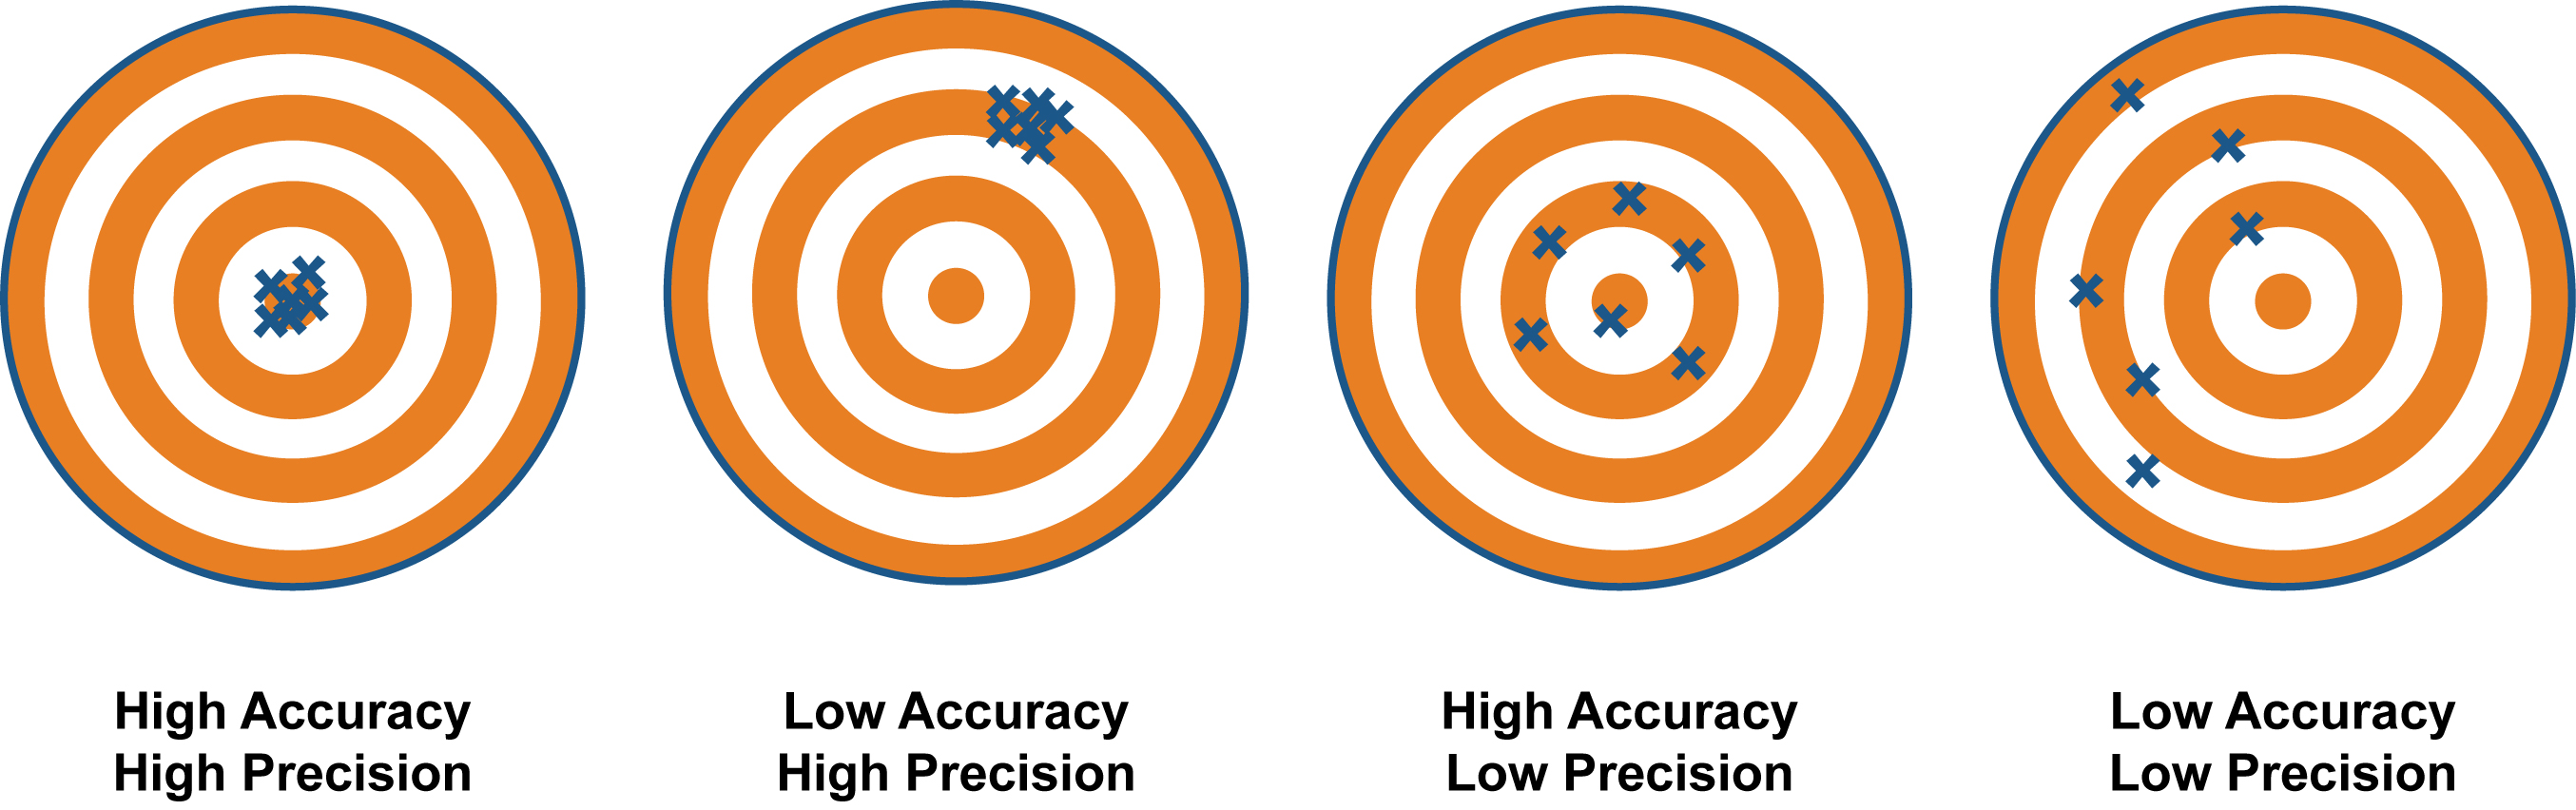
\includegraphics[width=\columnwidth]{acc_prec.jpeg}
\caption{``Measurements'' of varying accuracy and precision.
Credit:
\href{http://kaffee.50webs.com/Science/images/Accuracy-vs-precision1.jpg}{A.~Keller}.
%\href{http://kaffee.50webs.com/Science/images/Accuracy-vs-precision1.jpg}{http://kaffee.50webs.com/Science/images/Accuracy-vs-precision1.jpg}}
}
\end{centering}
\end{figure}

%\paragraph{}
Now let's say that the ruler we used was poorly manufactured, and the
true distance was $3\mathrm{cm}$. We would then say that the {\bf accuracy}
of the measurement was only $0.86\mathrm{cm}$. This ruler introduced a {\bf bias} into our data.
Note that it is sometimes
impossible to know how accurate a measurement is, since all you have
to compare it with may be other measurements, which are all slightly flawed.

%\paragraph{}
%Discuss the following questions with your group and
%\textbf{record some brief answers in your notebook}.
%
%\begin{itemize}
%\item How would you define ``experiment'' (the noun)? How does an
%experiment differ from a measurement?
%%\item Let's say you have two different methods of measuring a quantity
%%and can repeat each one many times. How would you determine which
%%method was ``better'' and what are your criteria?
%\item Let's say you have the value of a quantity as predicted by a
%theory and a set of measurements of that value from an
%experiment. How would you go about determining if the experimental
%results agree with the theory?
%\end{itemize}

Discuss the following as a group and \textbf{answer briefly in your notebook}.

\begin{enumerate}

\item How would you define the word \textit{experiment} (noun)? How does an
experiment differ from a measurement?
%\item Let's say you have two different methods of measuring a quantity
%and can repeat each one many times. How would you determine which
%method was ``better'' and what are your criteria?
\item Measurement uncertainty is sometimes broken down into ``random'' and ``systematic'' uncertainty. How would you define random and systematic uncertainty? Relate these terms to accuracy, precision, and bias as defined above.
\end{enumerate}

\section{Repeatable Measurements}

%\subsection{Measuring an object}
%
%%\paragraph{}
%To illustrate how to make a measurement, let's just do it!
%{\bf Write down each step in bold your lab notebook.}
%
%\begin{enumerate}
%\item {\bf Find something to measure}. It could be your notebook, the table, the
%hallway, just keep it on the $14^{th}$ floor.
%
%\item {\bf Now find something to measure your object with}. You want to
%pick the right tool for the job, so small objects should be measured
%with rulers and large objects should be measured with tape measures
%and yard sticks.
%
%\item It's always good to take a second {\bf BEFORE} you do anything in
%lab and estimate what your measurement or answer will be, and
%to try to think of any problems you will run into. Also be sure to
%describe what you're going to do before you do it. \textbf{What are you
%measuring? Is it consistently one size, or are some places bigger
%than others? What are you measuring with? How precise do you
%think you can be?} If you need to be creative to make your measurement,
%explain how you're going to do it.
%
%\item {\bf Now make your measurement, writing down the appropriate error}.
%Remember to write down the units! Describe how you took your measurement, or at least how you did it
%differently than you had planned.  Do the measurement a second time.
%\textbf{Is there any difference in your results?  Is this measurement accurate or precise? or both? Do you think there's a bias in your data?}
%
%\end{enumerate}

%\newpage
%\subsection{Measuring a height}

%\paragraph{}
%The uncertainties in your measurements thus far have been easy to
%determine because you should get the same values if you
%repeat the measurement. But what would you do if the measurement
%changed each time? To study this, you're going to find the time it
%takes for an object to fall from a height of your choosing.

%\paragraph{}
Let's measure how long it takes for an object to fall some distance in the Earth's gravitational field.
%You'll release an object from rest and measure its free-fall duration.
An object with initial velocity $v_i$ that experiences acceleration $a$ will travel a distance
\begin{equation}
x=v_i \times t \; + \; \frac{1}{2}a \times t^2
\end{equation}
over a time duration $t$. At Earth's surface, the gravitational acceleration $g$ is $9.8 \unit{m/s^2}$. Note that $v_i = 0$ if you are just dropping the object.

\begin{enumerate}

\item With your group, select an object and height from which you'll drop that object. \textbf{Measure the height and report it in your lab notebook.} How precisely can you measure this distance?
    %Report also a numerical value for your precision.

\item Before you start measuring, it's always good to estimate what value you expect to get. Use the distance equation to calculate how long your object should take to hit the floor once dropped. \textbf{Show your work.}

%Start with an order-of-magnitude estimate:
%\textbf{will the fall time be milliseconds, seconds, tens of seconds, or years?} 
\item Think about any problems you might encounter, or how your experimental design (e.g., choice of object, height) will affect your results. \textbf{Do you think your measurements will differ from your theoretical expectation? Why or why not?}

\item {\bf Now use a stopwatch to time an object falling from whatever height you picked. Repeat this measurement ten times}. The best way to present this is in a table. Remember to label columns and rows, and to report units, so that someone who was not present in our lab could understand what was done.
%to present this in your lab notebook is in the form of a table.
%Be sure to label the table, columns, and rows, and use units.

\item The stopwatch you used is probably precise to a hundredth of a second, but your measurements should be spread out over a larger range of values. \textbf{What different effects are contributing to the uncertainty in your measurement? How big is each effect?}

\item \textbf{Report the average of your measurements and error on your average} (subtract the absolute value of the distance from Question 2 from the average). \textbf{Show your work!} You can throw out measurements that you know are bogus, but be sure to justify it if you do. 
\item \textbf{As a group, report a numerical uncertainty for your measurements.} To keep it simple, the uncertainty can be calculated by subtracting the average from the highest and lowest value. Use whichever gives a larger uncertainty.

\item \textbf{Do your measurements agree or disagree with your theoretical expectation for the free-fall time? Explain.} You might visualize your measurements in some way to help make your case.


%You just calculated how long it \textit{should} take
%for an object to fall, and then measured the time it actually took. Do these values agree?
%In this class, when we ask does something agree, we aren't asking
%if the numbers are the same, we are asking \textit{ could} they
%be the same, considering the uncertainty in both values.

%\item In other words, {\bf do the range of values that each measurement could
%be overlap? Think of how to show this visually, and
%draw it in your notebook. Be sure to label everything.}

\end{enumerate}

\section{Measuring the height of Pupin}

%\subsection{Think like a theorist}
%%\paragraph{}
%Estimate the height of Pupin without making any measurements.
%Explain what steps you take to make that estimate,
%and also estimate the error on your estimated height.

% \setcounter{subsection}{7}
\subsection*{Design an experiment}

%\paragraph{}
\begin{enumerate}
\setcounter{enumi}{7}
    \item As a group, come up with (at least) two methods of measuring the height of Pupin from 5th floor to roof, and \textbf{record the procedure for each in your notebook. Which methods do you expect to work best and worst? Why? How will you determine the precision of your measurements?} Show your methods to your lab instructor before proceeding. 
\end{enumerate}
\subsection*{Make your measurement}

\begin{enumerate}
\setcounter{enumi}{8}
\item Once you have your instructor's approval, go measure the height of Pupin Hall! Repeat your experiment five times. \textbf{Determine a single value for the height of Pupin and the precision of that measurement.} After everyone has made their measurements we'll compare techniques and results.

\end{enumerate} 

\section{Conclusion}

\begin{enumerate}
\setcounter{enumi}{9}
\item Which technique do you think worked best, and why?

\item How did you decide which technique worked best?

%\item Determine a final value of the height of Pupin
%and the precision of that value.
\item What were your favorite and least favorite parts of this lab? 
\end{enumerate}


%\e

\end{document}





